%*----------- INTRODUÇÃO -------------------------------------------------------------
\begin{frame}[t]{Introdução} 
    \newcommand\vspaceintro{0.2cm}
    \transdissolve[duration=0.5]
    No Chile, até os anos 70 a agricultura era voltada, majoritariamente, ao fornecimento interno de produtos agrícolas não processados \cite{blueberryrecognition}\vspace{\vspaceintro}
    
    Atualmente, a agricultura é reponsável por 11\% do PIB (\$27 bilhões), representando 28\% do comércio e empregando 10\% da força de trabalho nacional\cite{ChilePIB:online} \vspace{\vspaceintro} 

    80\% das plantações de blueberry são do tipo "legacy blueberries"
    \vspace{-0.4cm}
    \begin{columns}[t]
        \column{.4\linewidth}
        \begin{center}
            %\centerline{
                \begin{figure}
                    %\roundpic[xshift=0cm,yshift=0cm]{5cm}{8cm}{dying-blueberry.jpg}
                    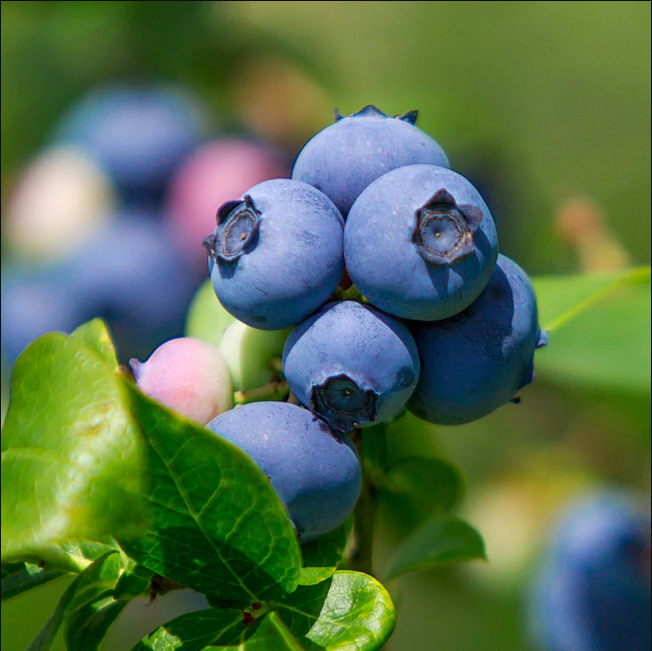
\includegraphics[width=0.5\textwidth]{blueberry-1.png}
                    %\caption{Pista de corrida \cite{agostini2007}}
                \end{figure}
            %}
        \end{center}

        \column{.4\linewidth}
        \begin{center}
            %\centerline{
                \begin{figure}
                    %\roundpic[xshift=0cm,yshift=0cm]{5cm}{8cm}{dying-blueberry.jpg}
                    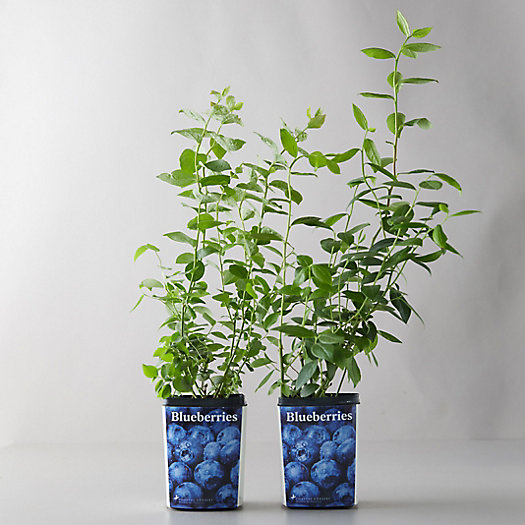
\includegraphics[width=0.5\textwidth]{blueberry-3.jpeg}
                    %\caption{Pista de corrida \cite{agostini2007}}
                \end{figure}
            %}
        \end{center}

        \column{.4\linewidth}
        \begin{center}
            %\centerline{
                \begin{figure}
                    %\roundpic[xshift=0cm,yshift=0cm]{5cm}{8cm}{dying-blueberry.jpg}
                    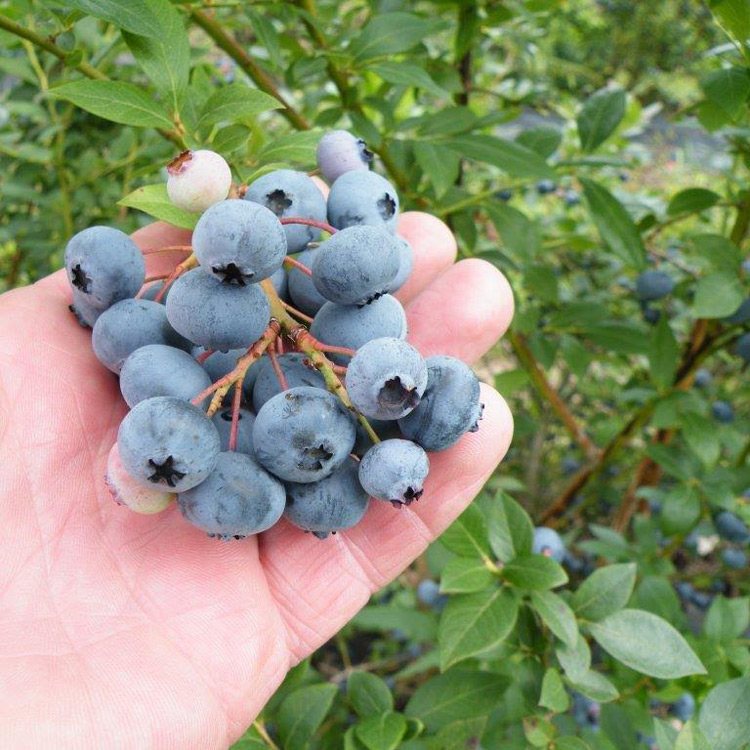
\includegraphics[width=0.5\textwidth]{blueberry-2.jpeg}
                    %\caption{Pista de corrida \cite{agostini2007}}
                \end{figure}
            %}
        \end{center}

    \end{columns}
%*----------- notes
    \note[item]{Notes can help you to remember important information. Turn on the notes option.}
\end{frame}
%-

%*----------- PROBLEMÁTICA -------------------------------------------------------------
\begin{frame}[t]{Problemática} 
    \transdissolve[duration=0.5]
    A agricultura chilena enfrenta os seguintes problemas:
    %\newline
        \begin{columns}[t]
            \column{.05\linewidth}
            \column{.4\linewidth}
                \begin{enumerate}
                    \item há previsões para o ano de 2030 sobre um abondono significativo dos trabalhadores na agricultura
                    \item no estágio de enraizamento durante as estações críticas ocorrem perdas superiores a 50\% dos brotos
                \end{enumerate}
            \column{.6\linewidth}
            \vspace{-0.5cm}
            \begin{center}
                \begin{figure}
                    \caption{Legacy Blueberry Seca}
                    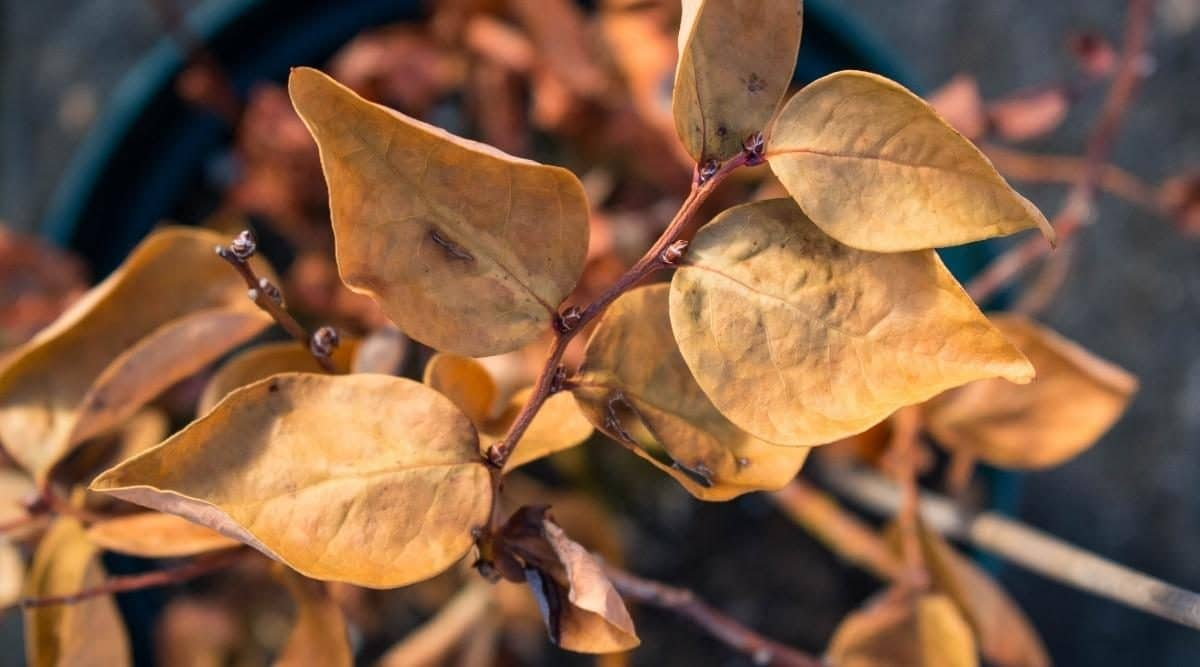
\includegraphics[width=0.7\textwidth]{dying-blueberry.jpg}
                \end{figure}
            \end{center}
        \end{columns}
%*----------- notes
    \note[item]{Notes can help you to remember important information. Turn on the notes option.}
\end{frame}
%-

%*----------- CONTEXTO -------------------------------------------------------------
\begin{frame}[t]{Contexto} 
    \newcommand\vspacecontexto{0.2cm}
    \transdissolve[duration=0.5]
    fgdfgdfgfd fgdfgdfgfd \vspace{\vspacecontexto}
    
    rttrd rdgd\vspace{\vspacecontexto} 
%*----------- notes
    \note[item]{Notes can help you to remember important information. Turn on the notes option.}
\end{frame}
%-